\subsection{26. Определение LR-грамматики, примеры LR и не LR-грамматик. Стековая аналогия определения (нет конфликтов).  Вопрос на отл: однозначность lr грамматики.}

\Def Грамматика называется LR(k) грамматикой, если LR-k таблица для этой грамматики строится корректно

\Def Для $\alpha \in (N \cup \Sigma)^*$ определим First($\alpha$) как:

First($\alpha$) = $\{a | \alpha\ \rightarrow  au, u \in \Sigma^*\} \cup \{\$\}I(\alpha \rightarrow \varepsilon$)
First($\alpha$) - первый символ, который может вывестись из $\alpha$.

Если $\alpha = a\gamma$, то First($\alpha$) = a

Если $\alpha$ = B$\gamma$, B $\rightarrow \varepsilon$, то First($\alpha$) = First(B) $\cup$ First($\gamma$)
\\
\\
\Def Грамматика называется LR(k) грамматикой, если из условий:
\begin{itemize}
    \item [1.] $S' \rightarrow \cdot \alpha A w \rightarrow \alpha \beta w$
    \item [2.] $S' \rightarrow \cdot \gamma B x \rightarrow \alpha \beta y $ где $\gamma$ - префикс $\alpha$, возможно, несобственный. x - суффикс $w$
    \item [3.] $First_k(w) = First_k(y)$
\end{itemize}
Что происходит в теминах алгоритма? На стеке сейчас лежат $\alpha \beta$ и мы смотрим, верно ли, что можно свернуть однозначно? Наличие двух одинаковых выводов говорит, что нет. То есть алгоритм стоит перед некоторой дилеммой. Можно свернуть А (по правилу $A \rightarrow \beta$) или прочитать что-то еще, и свернуть В(по правилу $B \rightarrow \nu_1 \beta \nu_2$). В первлм случае мы сворачиваем за один шаг, во втором случае - что-то еще сворачиваем, а уже после сворачиваем В.


Что делать в таких ситуациях? А ничего. мы говорим, что такого не допускаем :)


То есть мы говорим, что $\alpha A y = \gamma B x$, то есть $\alpha = \gamma, A = B$
\textbf{Конец определения} \\ \\
\textbf{Примеры LR грамматик}
\begin{itemize}
    \item Грамматика из примера к предыдущему билету
     \item 
     \begin{itemize}
         \item $S \rightarrow A$
         \item $A \rightarrow aA \; | \; b$
     \end{itemize}
     \begin{itemize}
        \item $S \rightarrow A \; | \; aB$
        \item $A \rightarrow aA \; | \; r$
        \item $B \rightarrow aB \; | \; m$
    \end{itemize}
\end{itemize}

Эти грамматики парсятся LR(0), и, соответственно, любой другой грамматикой

\textbf{Любая неоднозначная грамматика - не LR грамматика}
\\
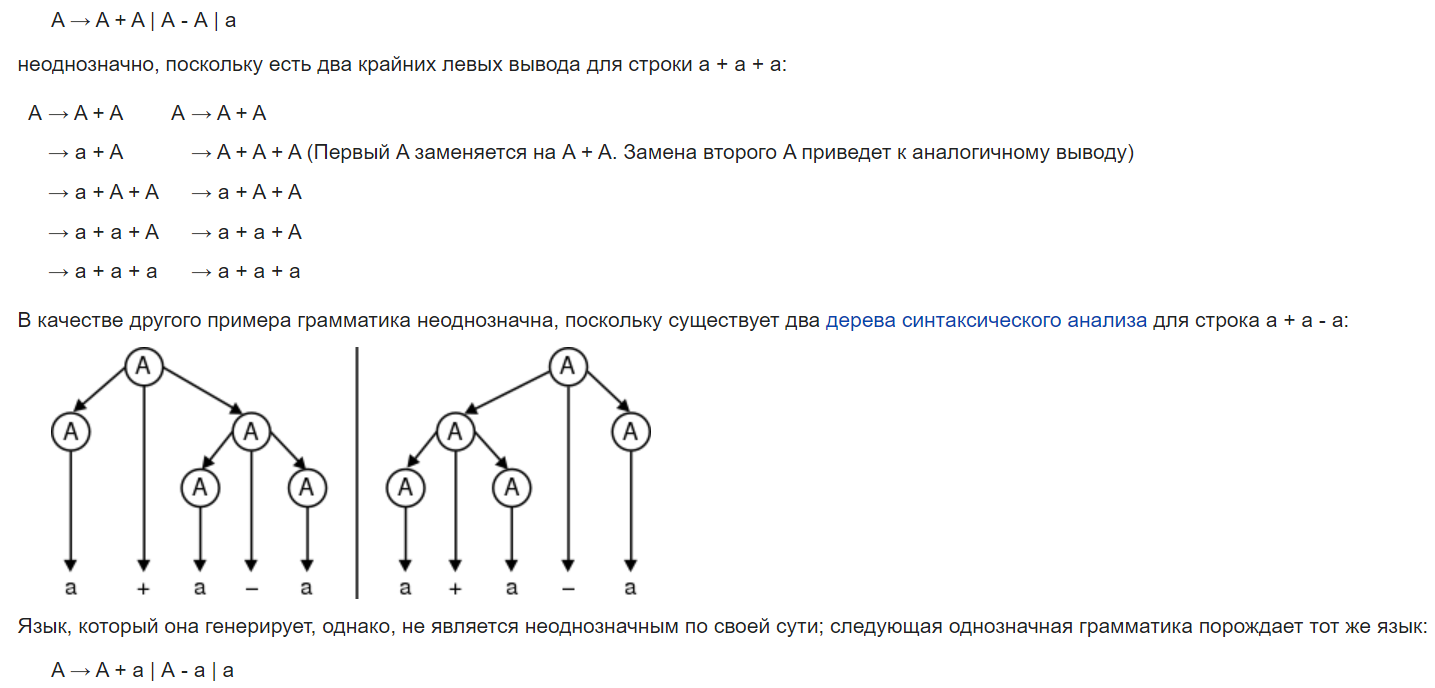
\includegraphics[width=17cm]{formal2.PNG}
\\
\textbf{Дополнительно. Пример грамматики LR(1), не являющейся LR(0) грамматикой}
\begin{itemize}
    \item $S' \rightarrow S$
    \item $S \rightarrow Bb$
    \item $S \rightarrow Cc$
    \item $B \rightarrow a$
     \item $C \rightarrow a$
\end{itemize}
LR(0) разбор
\begin{itemize}
    \item [0] \begin{itemize}
        \item $S' \rightarrow \cdot S$
    \item $S \rightarrow \cdot Bb$
    \item $S \rightarrow \cdot Cc$
    \item $B \rightarrow \cdot a$
     \item $C \rightarrow \cdot a$
    \end{itemize}
    \item [1] \begin{itemize}
        \item $B \rightarrow  a \cdot$
        \item $C \rightarrow a\cdot$
    \end{itemize}
    И все, есть два reduce. Мы не знаем, что делать. А в терминах вывода это означает, что мы могли открыть букву как  ab и как ac, и неважно, что слова разные, у нас уже конфликт в явном виде
\end{itemize}
LR(1) разбор
\begin{itemize}
        \item [0] \begin{itemize}
        \item $S' \rightarrow \cdot S, \$ $
    \item $S \rightarrow \cdot Bb,\$ $
    \item $S \rightarrow \cdot Cc \$$
    \item $B \rightarrow \cdot a, b$
     \item $C \rightarrow \cdot a, c$
    \end{itemize}
    \item [1] \begin{itemize}
        \item $B \rightarrow  a \cdot, b$
        \item $C \rightarrow a\cdot, c$
        \\
        Тут такого противоречия нет, так как мы подсмотрели следующие буквы и поняли, что это соответственно будут reduce(3) и  reduce(4), то есть сейчас мы эти ситуации отличаем
    \end{itemize}
\end{itemize}

\par \textbf{Однозначность LR-грамматики (на отл):}
\begin{figure}[h]
\center{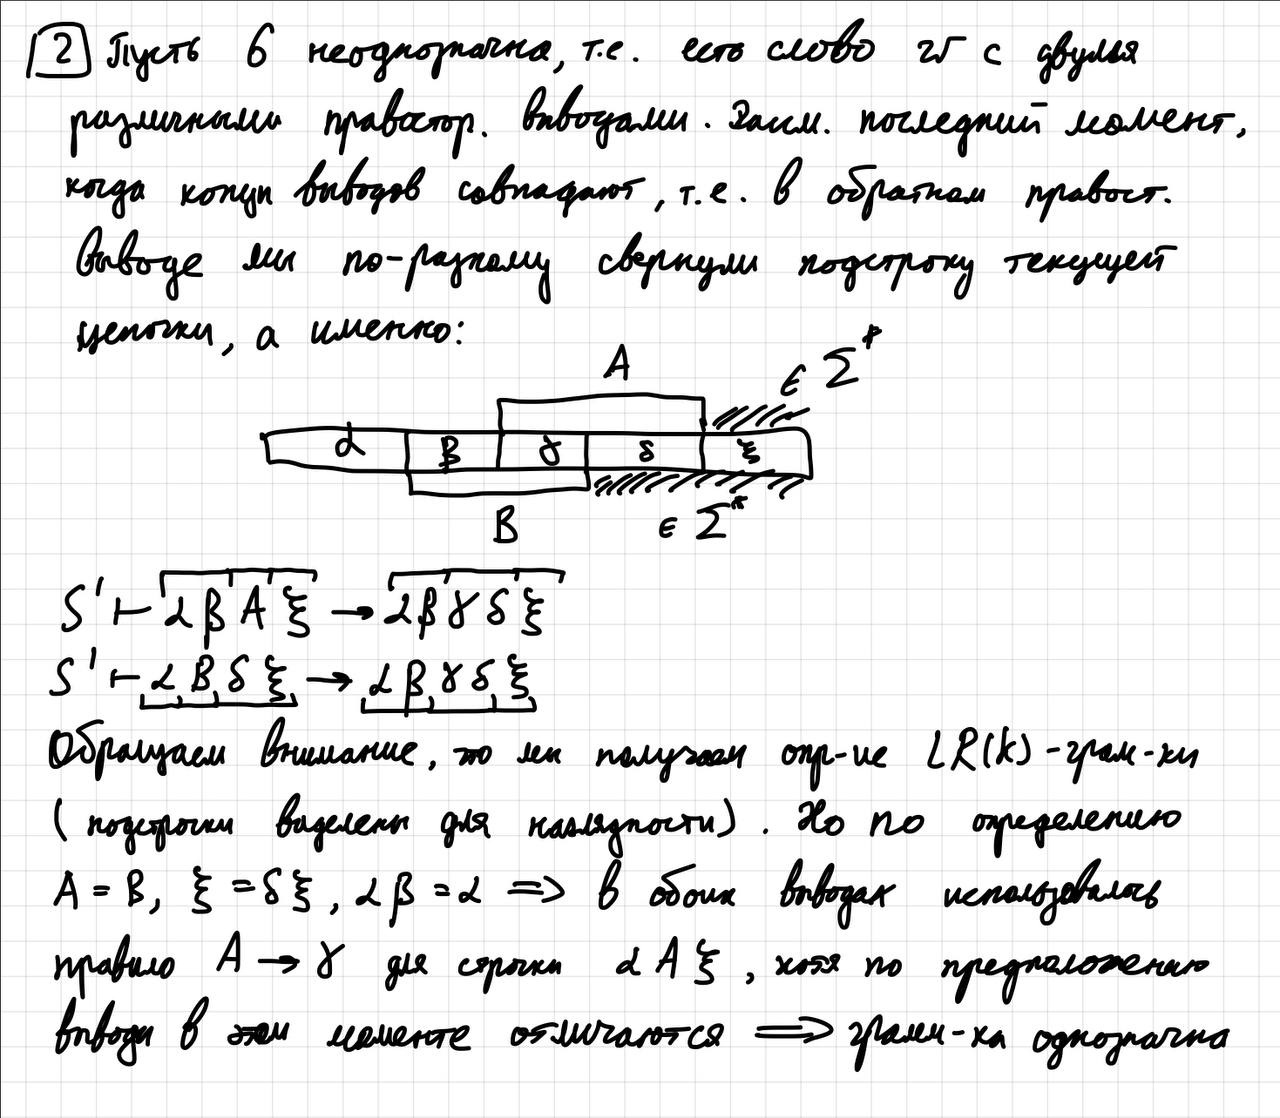
\includegraphics[scale=0.35]{images/LR-unambiguity.jpg}}
\end{figure}